\documentclass[tikz]{standalone}

\begin{document}
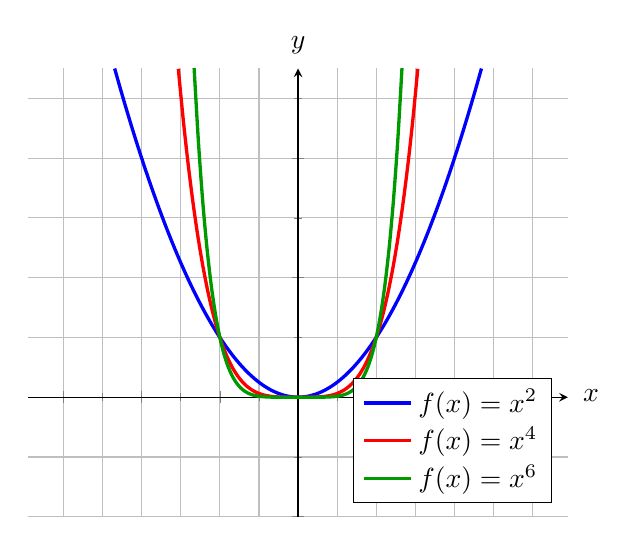
\begin{tikzpicture}
    \begin{axis}[%
        xlabel=$x$, ylabel=$y$, legend pos=south east,
        grid=both, xmin=-3.45, xmax=3.45, ymin=-2, ymax=5.5,
        axis lines = middle,
        minor x tick num=1, minor y tick num=1,
        xlabel style = {at={(axis description cs:1.01,0.27)},anchor=west},
        ylabel style = {at={(axis description cs:0.5,1.01)},anchor=south},
        xticklabels = {}, yticklabels={},
    ]
    \addplot[blue, very thick, smooth, samples=50, domain=-2.345:2.345] plot {x^2};
    \addplot[red, very thick, smooth, samples=50, domain=-1.531:1.531] plot {x^4};
    \addplot[green!60!black, very thick, smooth, samples=50, domain=-1.329:1.329] plot {x^6};
    \legend{$f(x)=x^2$,$f(x)=x^4$,$f(x)=x^6$}
    \end{axis}
\end{tikzpicture}
\end{document}
